\documentclass[a4paper,11pt]{article}
\usepackage[utf8]{inputenc}
\usepackage[greek]{babel}
\usepackage[LGR]{fontenc}
\usepackage{multirow}
\usepackage{amsmath}
\usepackage{bm}
\usepackage{enumerate}
\usepackage{enumitem}
\usepackage{moreenum}
\usepackage{graphicx}
\usepackage{ragged2e}

\newcommand{\lt}{\latintext}
\newcommand{\gt}{\greektext}

\begin{document}


\title{Πρώτη Εργασία στην Αριθμητική Ανάλυση}
\author{Παρμενίων Χαριστός \\ ΑΕΜ: 3173}
\date{1 Νοεμβρίου 2020}
\maketitle

\section{Πρώτη Άσκηση}

\begin{center}
{\scriptsizeΑ\footnotesizeΒ\smallΓ\normalsizeΔ\largeΕ\LargeΖ\LARGEΗ\hugeΘ\HugeΙ\hugeκ\LARGEλ\Largeμ\largeν\normalsizeξ\smallο\footnotesizeπ\scriptsizeρ\tinyς}
\end{center}

\section{Δεύτερη Άσκηση}

\begin{center}
\begin{large}
\lt{\textnormal{Normal} \textit{Italics} \textbf{Bold}\newline
\emph{Emphasized} \underline{\textnormal{Underlined}}}
\end{large}
\end{center}

\section{Τρίτη Άσκηση}

$$a^2=b^2+c^2$$
 $$e^{i\pi}=-1$$
$$\pi=\frac{c}{d}$$
$$\frac{d}{dx}\int_{a}^xf(s)ds=f(x)$$
$$f(x)=\sum_{i=0}^\infty \frac{f^{(i)}(0)}{i!}x^i $$
\begin{center}
\lt{  \textbf{Ax=b}}
\end{center}
$$\| x+y \| \le \|x \|+\|y\|$$  
\begin{equation}
\mathbf{I}=\begin{pmatrix} 1 & 0 & 0 & 0\\ 0 & 1 & 0 & 0\\0 & 0 & 1 & 0\\0& 0 &0 &1 \end{pmatrix}
\end{equation}
\begin{equation}
\mathbf{I}=\begin{bmatrix} 1 & 0 & 0 & 0\\ 0 & 1 & 0 & 0\\0 & 0 & 1 & 0\\0& 0 &0 &1  \end{bmatrix}
\end{equation}
\begin{equation}
\mathbf{I}=\begin{Bmatrix}1 & 0 & 0 & 0\\ 0 & 1 & 0 & 0\\0 & 0 & 1 & 0\\0& 0 &0 &1 \end{Bmatrix} ,\quad\mathbf{I}=\begin{vmatrix}  1 & 0 & 0 & 0\\ 0 & 1 & 0 & 0\\0 & 0 & 1 & 0\\0& 0 &0 &1 \end{vmatrix},\quad\mathbf{I}=\begin{Vmatrix} 1 & 0 & 0 & 0\\ 0 & 1 & 0 & 0\\0 & 0 & 1 & 0\\0& 0 &0 &1 \end{Vmatrix} 
\end{equation}

\section{Τέταρτη Άσκηση}


\begin{center}
  \begin{tabular}{  l  c  r }
    Τέφας & 2 & 3 \\ 
    Πήτας & 5 & 6 \\ 
    Λάσκαρης & 8 & 9 \\
  \end{tabular}
\end{center} 
\bigskip

\begin{center}
  \begin{tabular}{ | l | c | r | }
    Κοτρόπουλος & 6 & 3 \\ 
    Πήτας & 5 & 6 \\ 
    Νικολαίδης & 8 & 9 \\
  \end{tabular}
\end{center}
\bigskip

\begin{center}
  \begin{tabular}{ | l | c | r | }
    \hline
    1 & 2 & 3 \\ \hline
    4 & 5 & 6 \\ \hline
    7 & 8 & 9 \\
    \hline
  \end{tabular}
\end{center}
\bigskip

\begin{center}
  \begin{tabular}{ | l | c | r | }
    \hline
    1 & 2 & 3 \\ \hline
    4 & 5 & 6 \\ \hline
    7 & 8 & 9 \\
    \hline
  \end{tabular}
\end{center}
\bigskip

\begin{center}
\begin{tabular}{l*{6}{c}r}
\begin{tabular}{ |l|l|l| }
\hline
\multicolumn{3}{ |c| }{Μέλη ΔΕΠ Πληροφορικής} \\
\hline
Λέκτορες &  \lt VD & Δραζιώτης Κωνσταντίνος \\ \hline
\multirow{2}{*}{Επίκουροι} & \lt LN & Λάσκαρης Νικόλαος\\
 & \lt TG & Τσουμάκας Γρηγόριος\\ \hline
\multirow{3}{*}{Αναπληρωτές} & \lt TA & Τεφάς Αναστάσιος\\
 & \lt PN & Πλέρος Νίκος \\
 & \lt PA & Παπαδόπουλος Απόστολος \\ \hline
\multirow{3}{*}{Καθηγητές} & \lt KC & Κοτρόπουλος Κωνσταντίνος \\
 & \lt PI & Πίτας Ιωάννης\\
 &  \lt VI & Βλαχάβας Ιωάννης\\
\hline
\end{tabular}
\end{tabular}
\end{center}

\section{Πέμπτη Άσκηση}

\begin{itemize}  
\item Τέφας
\item Μπουζάς
\item Μπρούζα
\item Λάσκαρης
\item Κοτρόπουλος
\item Πήτας
\item Νικολαΐδης
\end{itemize}

\begin{enumerate}
\item Τέφας
\item Μπούζας
\item Μπρούζα
\item Λάσκαρης
\item Κοτρόπουλος
\item Πήτας
\item  Νικολαΐδης
\end{enumerate}

\begin{enumerate}[label=\textbf(\textbf{\greek*}\textbf)]
\item Τέφας
\item Μπουζάς
\item Μπρούζα
\item Λάσκαρης
\item Κοτρόπουλος
\item Πήτας
\item Νικολαϊδης
\end{enumerate}

\section{Έκτη Άσκηση}

\Centering
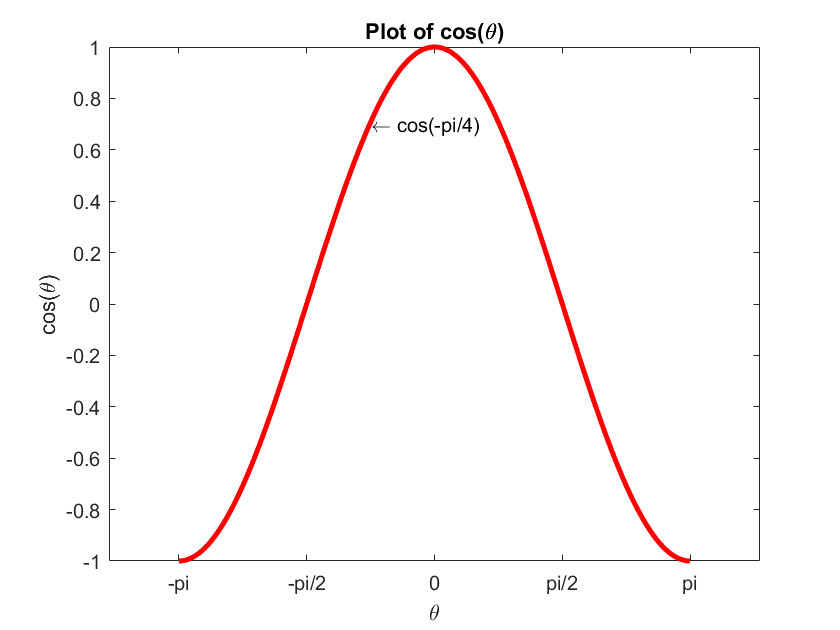
\includegraphics[height = 90mm]{cos.png}
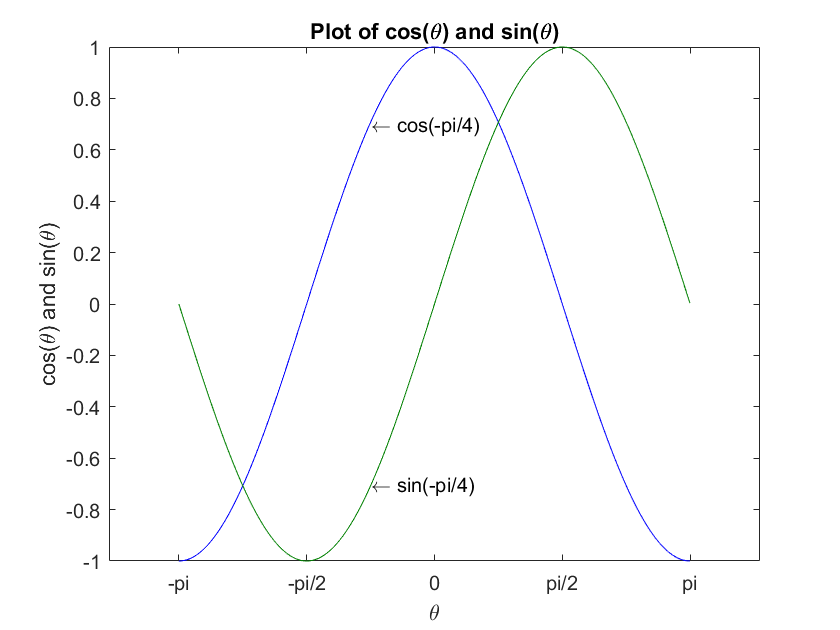
\includegraphics[height = 90mm]{cos_sin.png}



\end{document}
